

\documentclass[JIP]{ipsj_v2/UTF8/ipsj}

\usepackage[dvipdfmx]{graphicx}
\usepackage{latexsym}
\usepackage{amssymb}
\usepackage{float}
\usepackage{enumerate,cite,url}
\usepackage{listings,jlisting}
\lstset{%
    language={c},%
    basicstyle={\small},%
    identifierstyle={\small},%
    commentstyle={\footnotesize\itshape},%
    keywordstyle={\small},%\bfseries},%
    ndkeywordstyle={\small},%
    stringstyle={\small\it},
    frame={tb},
    breaklines=true,
    columns=[l]{fullflexible},%
    numbers=left,%
    xrightmargin=0zw,%
    xleftmargin=3zw,%
    numberstyle={\scriptsize},%
    stepnumber=1,
    numbersep=1zw,%
    lineskip=-0.5ex%
}

\def\Underline{\setbox0\hbox\bgroup\let\\\endUnderline}
\def\endUnderline{\vphantom{y}\egroup\smash{\underline{\box0}}\\}
\def\|{\verb|}


\setcounter{volume}{22}% vol22=2014
\setcounter{number}{4}% 1=Jan., 2=Apr., 3=July, 4=Oct.
\setcounter{page}{1}


\received{2014}{3}{4}
%\rereceived{2011}{10}{1}   % optional
%\rerereceived{2011}{10}{31} % optional
\accepted{2014}{8}{1}



\usepackage[varg]{txfonts}%%!!
\makeatletter%
\input{ot1txtt.fd}
\makeatother%

\begin{document}

\title{Component-based Software Development Framework \\for Embedded IoT Devices(仮)}

\affiliate{OSAKA}{Graduate School of Engineering Science, Osaka University}
\affiliate{NAGOYA}{Graduate School of Informatics, Nagoya University}
\affiliate{OKUMA}{OKUMA Corporation}

\author{Takuro Yamamoto}{OSAKA}
\author{Takuma Hara}{NAGOYA}
\author{Takuya Ishikawa}{NAGOYA}
\author{Hiroshi Oyama}{OKUMA}
\author{Hiroaki Takada}{NAGOYA}
\author{Takuya Azumi}{OSAKA}


\begin{abstract}

\end{abstract}

\begin{keyword}

\end{keyword}

\maketitle

%1
\section{Introduction}
\label{sec:Introduction}

The Internet of Things (IoT) is an essential next evolutionary step for the Internet \cite{par:IoTComputing} in which various items and platforms, for example, wearable devices and smart devices, will be connected via the Internet to further enrich people's lives.
The IoT uses embedded systems such as data sensors and controlling actuators as elemental constituents, and they must demonstrate high quality and high performance.
This requirement has led to an increase in their complexity and scale; moreover, these systems need to have low production costs and short development cycles.

Complex and large-scale software systems can be developed efficiently by using component-based techniques \cite{par:Crnkovic}, \cite{par:CBD}.
Component-Based Development (CBD) is a design technique that can be applied to reusable software development.
Verification of component-based systems has been extensively researched \cite{par:Blaming}, \cite{par:Verification}.
Individual component diagrams enable the visualization of an entire system.
In addition, component-based systems are flexible with regard to extensibility and specification changes.
The TOPPERS embedded component system (TECS) \cite{par:TECS}, AUTOSAR \cite{url:AUTOSAR}, and SaveCCM \cite{par:SAVEapproach} are typical CBD tools for embedded systems.

In addition, scripting languages, such as Ruby, JavaScript, Perl, Python, and Lua, offer efficient approaches to software development.
Currently, most embedded software are programmed in C language.
However, development in C language results in large code size, incurs high costs, and requires significant development time.
In contrast, the use of scripting languages improves the efficiency of software engineering and can shorten the development period because it is relatively easy to reuse scripts. 

For embedded systems, real-time properties, such as estimation of worst-case execution time, are very important.
Although scripting languages are easy to use and read, their execution requires more time than that required by the codes written in C.
Therefore, applying scripting languages to embedded systems is difficult.
To address the above limitation, ``mruby on TECS,'' a component-based framework for running script programs, has been proposed \cite{par:mrubyonTECS}.
This framework integrates two technologies, i.e., mruby, which is a lightweight implementation of Ruby for embedded systems \cite{par:mruby}, \cite{url:mruby}, and TECS, which is a component-based framework for embedded systems \cite{par:TECS}, \cite{url:TOPPERS}.

This paper proposes an extended framework of mruby on TECS that can be applied to embedded network software development for IoT devices.
In the proposed framework, a component-based TCP/IP protocol stack, TINET+TECS \cite{par:TINET+TECS}, is comprised, and it is possible to utilize TINET function from mruby programs.

TINET is a compact TCP/IP protocol stack for embedded systems \cite{url:TINET}.
TINET comprises many complex source codes, i.e., it contains many files and defines many macros, which can be problematic for software developers seeking to maintain, extend, and analyze the software.
TINET+TECS is a componentized TIENT with TECS to improve the configurability and scalability of TCP/IP software.

In addition, this paper proposes a component-based dynamic memory allocator, TLSF+TECS. 
TLSF is a dynamic memory allocator for real-time systems, which can always run with $O(1)$ and improve memory usage efficiency by deviding memory blocks in two stages.
In the current version of TLSF, memory contention may occur when multiple threads run at the same time.
TLSF+TECS is a componentized TLSF memory allocator, which can be thread-safe allocator because each component has its own heap area.



{\bf Contributions}: The proposed framework provides the following contributions.
\begin{enumerate}
\item {\bf :}
\item {\bf :}
\item {\bf :}
\item {\bf :}
\end{enumerate}

{\bf Organization}: The remainder of this paper is organized as follows.
Section \ref{sec:System Model} introduces the system model of the proposed framework and the basic technologies, i.e., mruby, TECS, and mruby on TECS.
Section \ref{sec:Proposed Framework} describes the design and implementation of the proposed framework, including TINET+TECS and TLSF+TECS.
Section \ref{sec:Evaluation} evaluates the proposed framework.
Related work is discussed in Section \ref{sec:Related Work}.
Conclusions and suggestions for future work are presented in Section \ref{sec:Conclusion}.


%2
\section{System Model}
\label{sec:System Model}

This section describes the system model of the proposed framework, including basic technologies such as TECS.
The system model of the proposed framework is shown in Fig.\ref{fig:SystemModel}.

The proposed framework is an extension of mruby on TECS framework \cite{par:mrubyonTECS}\cite{par:mrubyonTECS2}, and utilizes two technologies: mruby and TECS.
In this section, mruby (\ref{sec:mruby}), TECS (\ref{sec:TECS}), and mruby on TECS framework (\ref{sec:mrubyonTECS}) are described.

\begin{figure}[t]
    \centering
    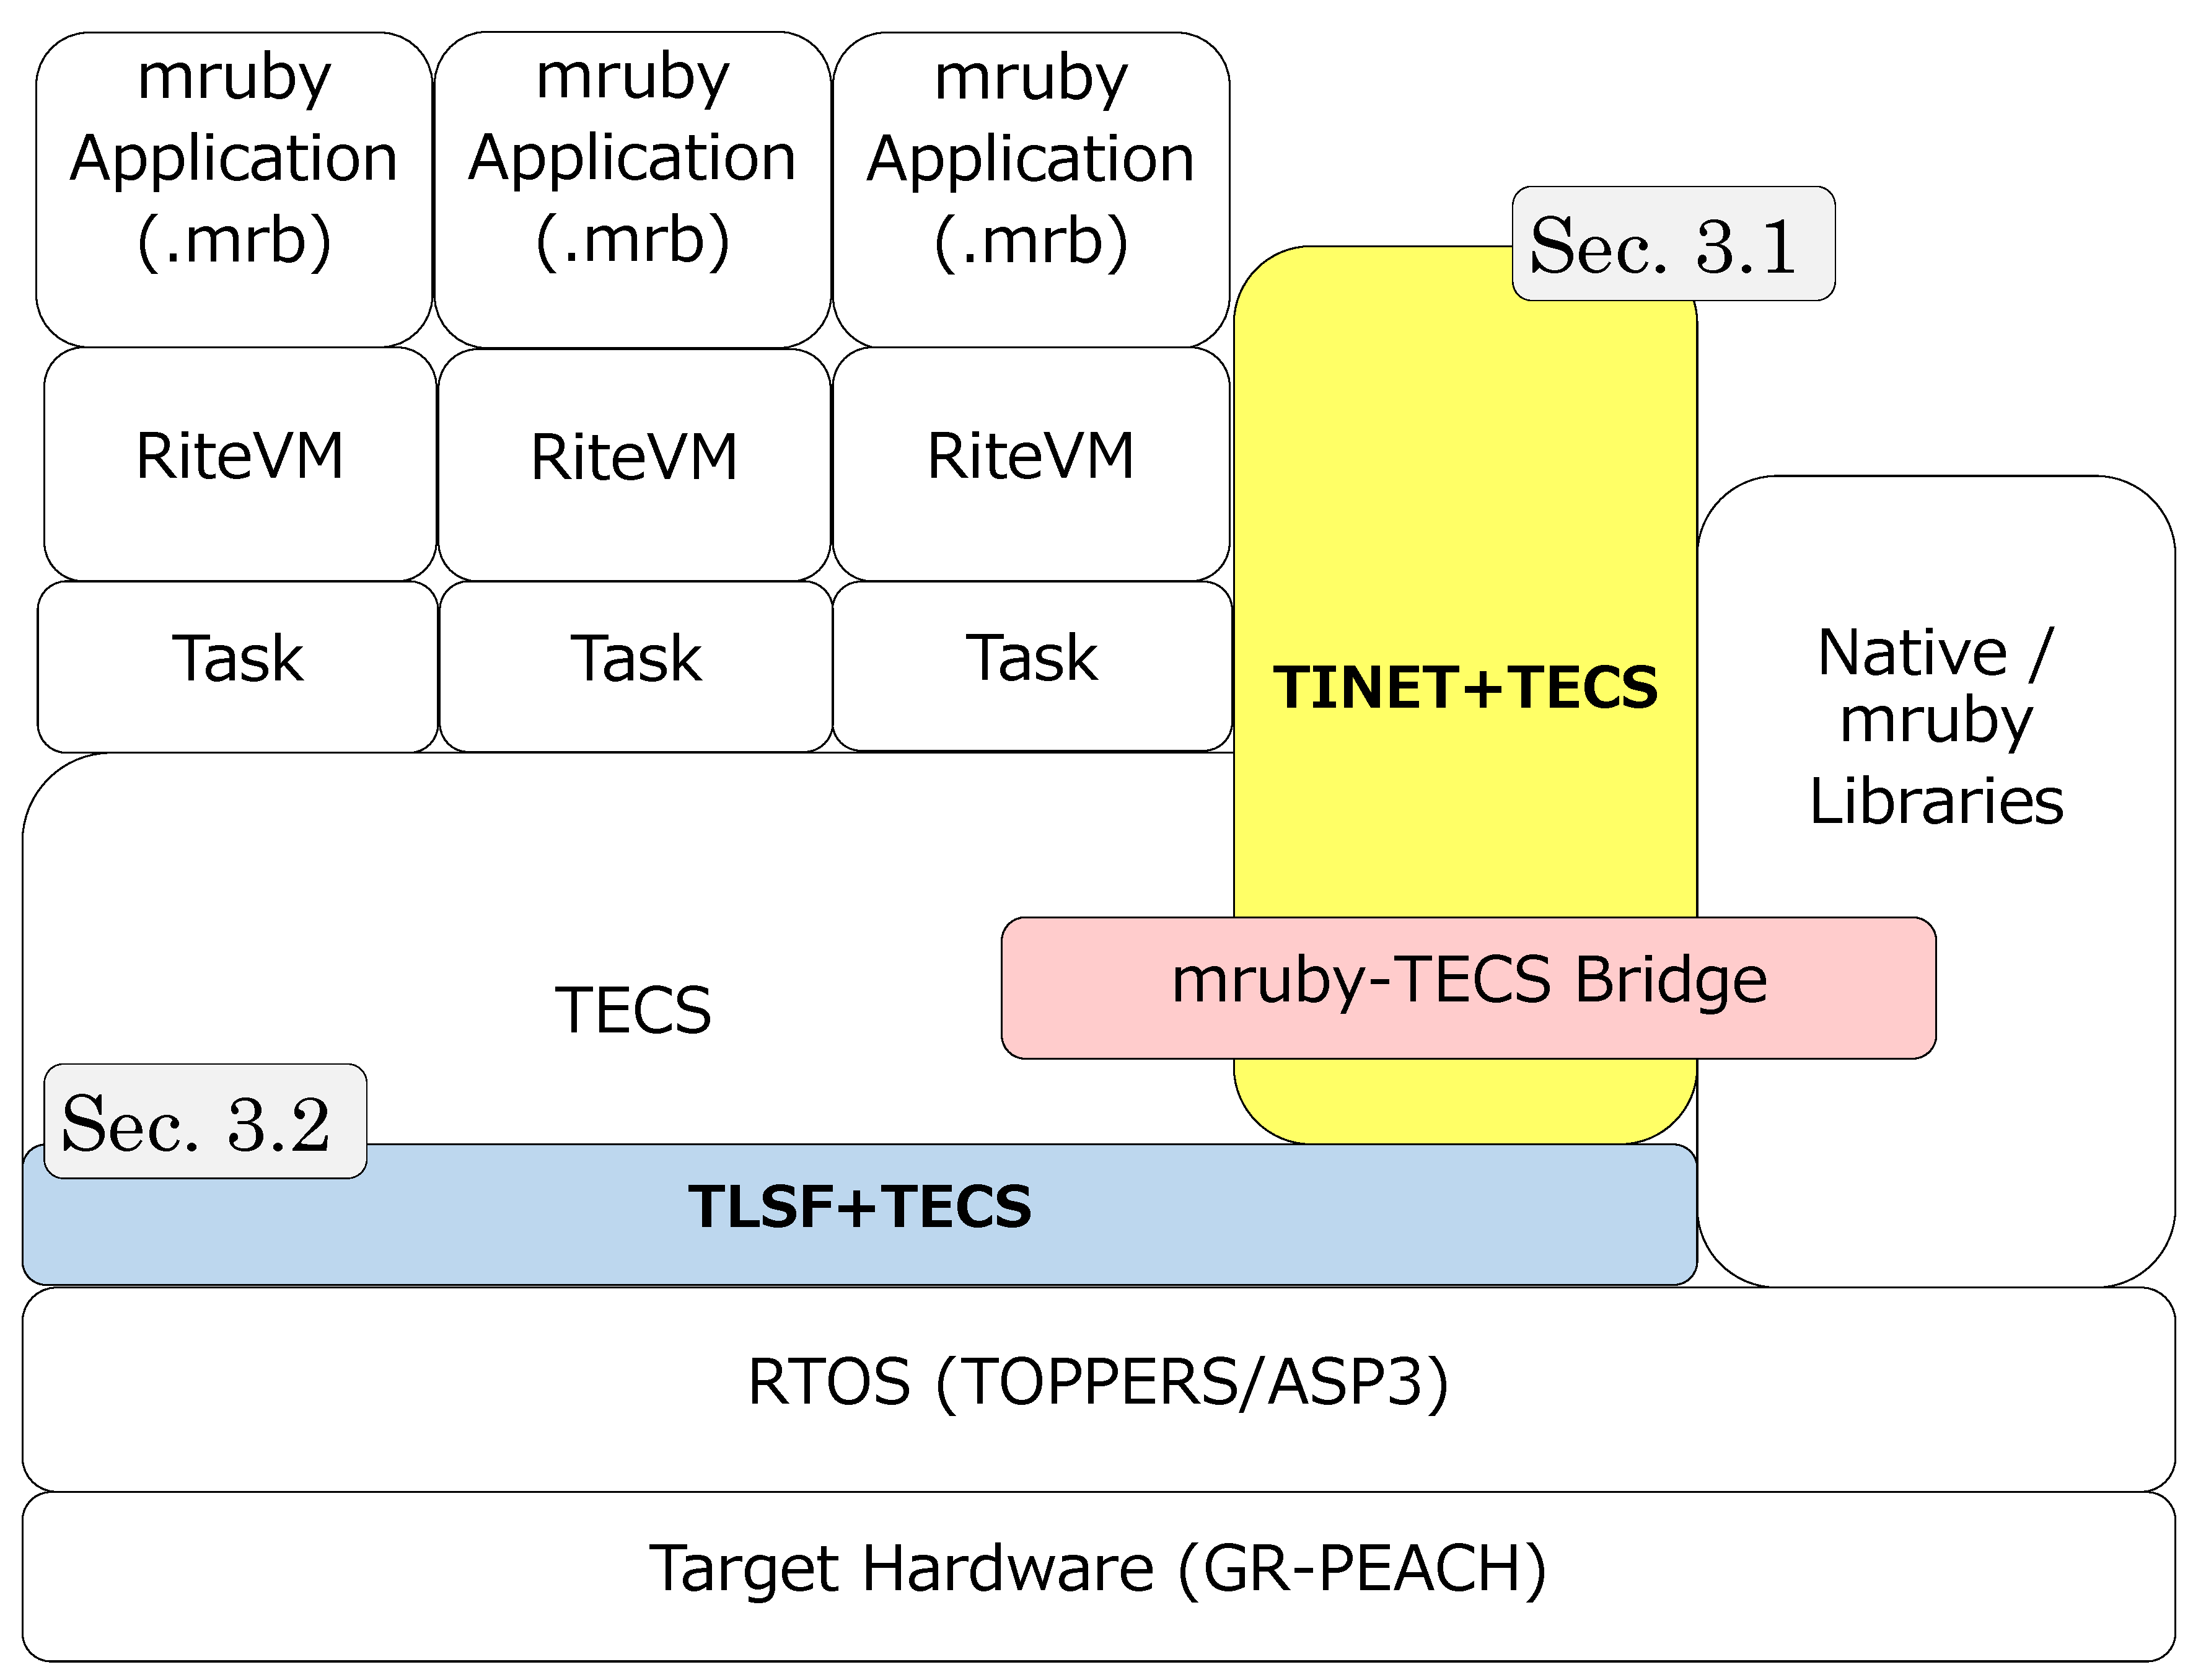
\includegraphics[width=8.0cm,clip]{figure/SystemModel.pdf}
    \caption{System model of the proposed framework}
    \label{fig:SystemModel}
\end{figure}

\subsection{mruby}
\label{sec:mruby}


\subsection{TECS}
\label{sec:TECS}

TECS is a component system suitable for embedded systems.
TECS can increase productivity and reduce development costs due to improved reusability of software components.
TECS also provides component diagrams, which help developers visualize the overall structure of a system.

In TECS, component deployment and composition are performed statically.
Consequently, connecting components does not incur significant overhead and memory requirements can be reduced.
TECS can be implemented in C, and demonstrates various feature such as source level portability and fine-grained components.

\begin{figure}[t]
    \centering
    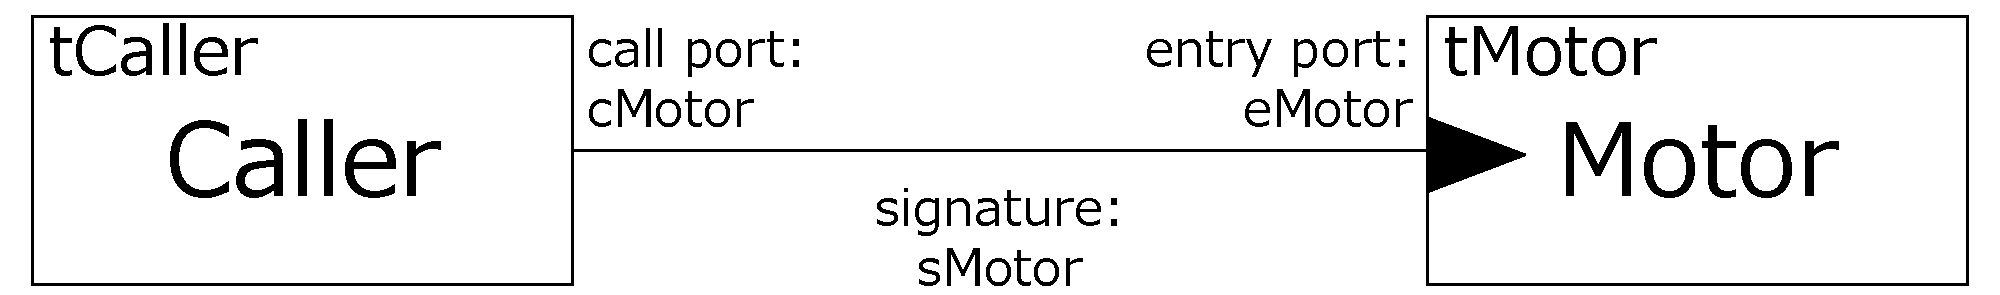
\includegraphics[width=6.5cm,clip]{figure/component_diagram.pdf}
    \caption{Component Diagram}
    \label{fig:component}
\end{figure}

\subsubsection{Component Model}
Fig.\ref{fig:component} shows a component diagram.
A {\it cell}, which is an instance of a component in TECS, consists of {\it entry} ports, {\it call} ports, attributes and internal variables.
An {\it entry} port is an interface that provides functions to other {\it cell}s, and a {\it call} port is an interface that enables the use of other {\it cell}'s functions.
A {\it cell} has one or more {\it entry} ports and {\it call} ports.
{\it Cell} functions are implemented in C.

The type of {\it entry}/{\it call} port is defined by a {\it signature}, which is a set of functions.
A {\it signature} is the interface definition of a {\it cell}.
The {\it cell}'s  {\it call} port can be connected to the {\it entry} port of another {\it cell} by the same {\it signature}.
Here, {\it celltype} defines one or more {\it call}/{\it entry} ports, attributes, and internal variables of a {\it cell}.


\subsubsection{Component Description}
In TECS, components are described by {\it signature}, {\it celltype}, and build written in component description language (CDL).
% TECS code is written in CDL (component description language) file.
These components are described as follows.

\begin{description}
    \item[{\bf Signature Description}]\mbox{}\\
        The {\it signature} defines a {\it cell} interface.
        The {\it signature} name follows the keyword {\it signature} and takes the prefix ``s'' e.g., sMotor (Fig.\ref{signature}).
        In TECS, to clarify the function of an interface, specifiers such as [in] and [out] are used, which represent input and output, respectively.
\begin{figure}[t]
\centering
\begin{lstlisting}
signature sMotor {
    int32_t getCounts( void );
    ER resetCounts( void );
    ER setPower( [in]int power );
    ER stop( [in] bool_t brake );
    ER rotate( [in] int degrees,
               [in] uint32_t speed_abs,
                [in] bool_t blocking );
    void initializePort( [in]int32_t type );
};
\end{lstlisting}
\caption{Signature Description}
\label{signature}
\end{figure}
    \item[{\bf Celltype Description}]\mbox{}\\
        The {\it celltype} defines {\it entry} ports, {\it call} ports, attributes, and variables.
        A {\it celltype} name with the prefix ``t'' follows the keyword {\it celltype}, e.g., tCaller (Fig.\ref{celltype}).
        To define {\it entry} ports, a {\it signature}, e.g., sMotor, and an {\it entry} port name, e.g., eMotor, follow the keyword {\it entry}.
        {\it Call} ports are defined similarly.
        Attributes and variables follow the keywords {\it attr} and {\it var}, respectively.
\begin{figure}[t]
\centering
\begin{lstlisting}
celltype tCaller {
    call sMotor cMotor;
};
celltype tMotor {
    entry sMotor eMotor;
    attr {
        int32_t port;
    };
    var {
        int32_t currentSpeed = 0;
    };
};
\end{lstlisting}
\caption{Celltype Description}
\label{celltype}
\end{figure}
    \item[{\bf Build Description}]\mbox{}\\
        The build description is used to instantiate and connect {\it cell}s.
        Fig.\ref{build} shows an example of a build description.
        A {\it celltype} name and {\it cell} name, e.g., tMotor and Motor, respectively, follow the keyword {\it cell}.
        To compose {\it cell}s, a {\it call} port, {\it cell}'s name, and an {\it entry} port are described in that order.
        In Fig.\ref{build}, {\it entry} port eMotor in {\it cell} Motor is connected to {\it call} port cMotor in {\it cell} Caller.
        {\it C\_EXP} calls macros defined in C files.

\begin{figure}[t]
\centering
\begin{lstlisting}
cell tMotor Motor {
    port = C_EXP("PORT_A");
};
cell tCaller Caller {
    cMotor = Motor.eMotor;
};
\end{lstlisting}
\caption{Build Description}
\label{build}
\end{figure}

\end{description}

\subsubsection{Development Flow}

\begin{figure}[t]
    \centering
    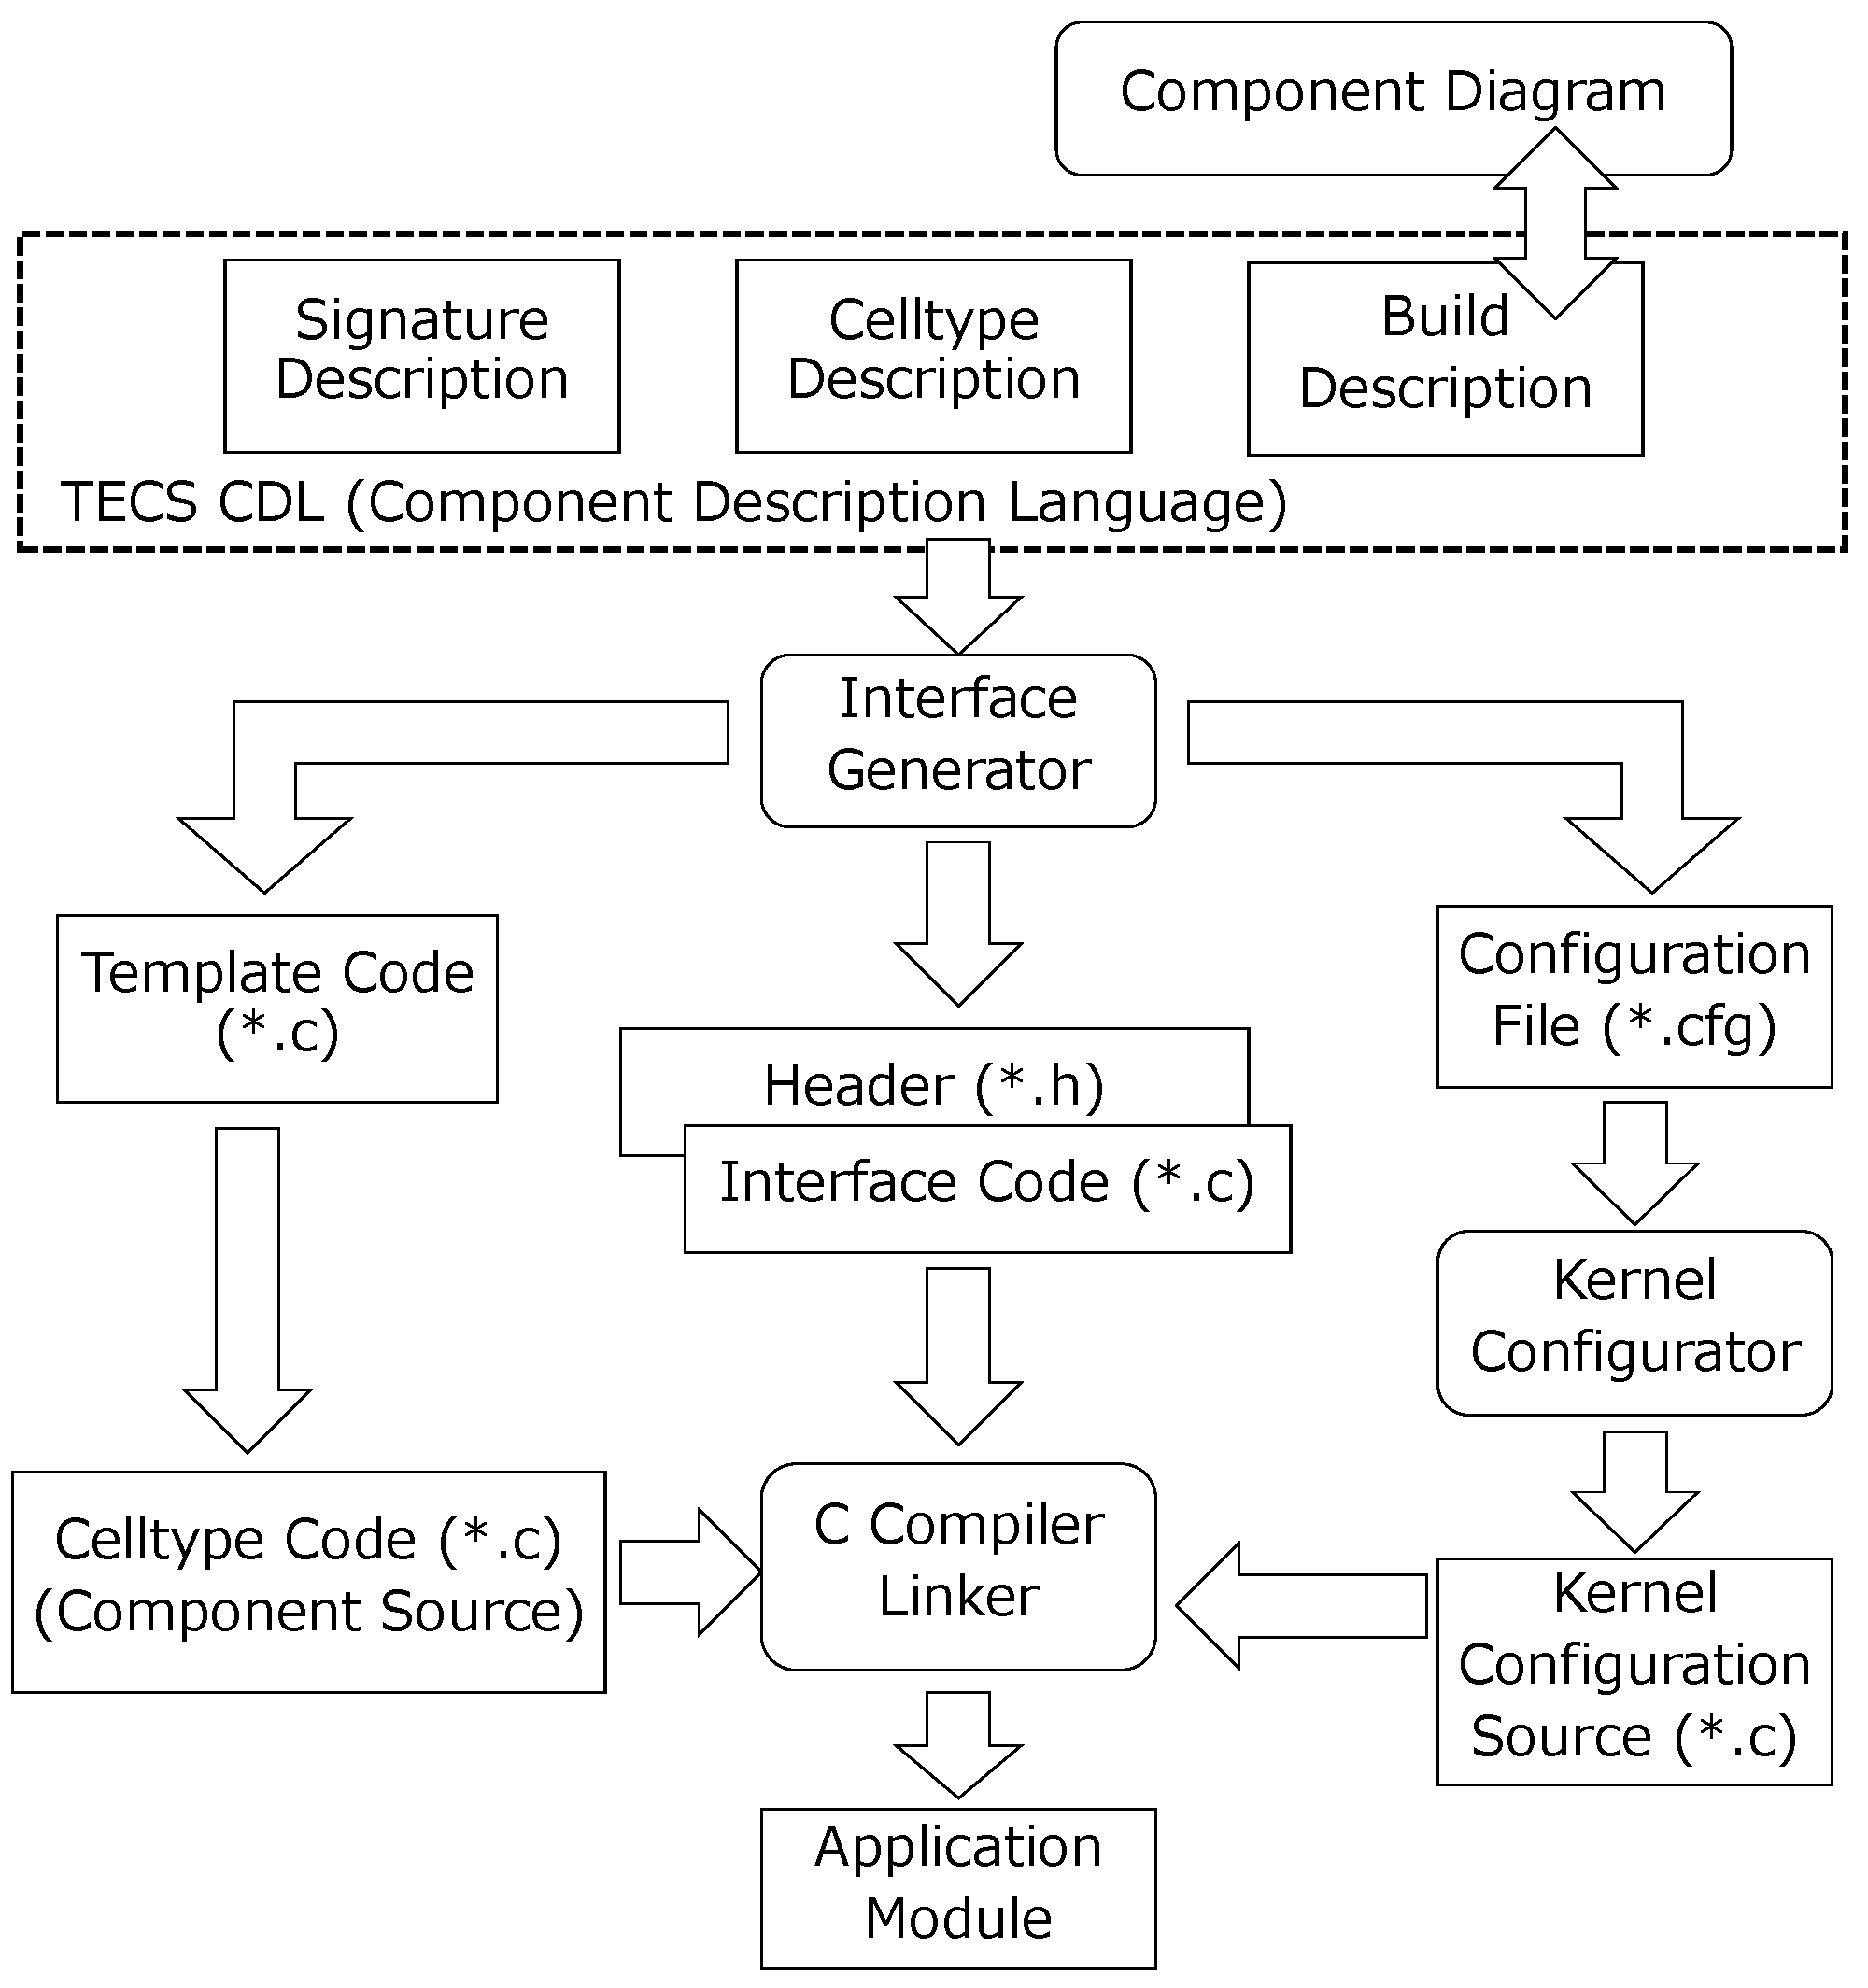
\includegraphics[width=8cm,clip]{figure/TECSFlow.pdf}
    \caption{Development flow using TECS}
    \label{fig:TECSFlow}
\end{figure}

Fig.\ref{fig:TECSFlow} shows the development flow using TECS.
TECS generator generates the interface code (.H and .C) and the configure file of the RTOS (.cfg) from the CDL file.

Software developers using TECS can be divided into component designers and application developers.
Component designers define signatures, which are interfaces between cells, and celltypes, which are types of cells.
Using the template code generated from the CDL file in which these are defined, component designers implement the functions and behaviors of the component in C language.
The source code implementing the function of the component is called a celltype code.
Application developers develop applications by using component diagrams and predefined celltype to connect cells with build description.
An application module is generated by compiling and linking the header, the interface code, and the celltype code.

\subsection{mruby on TECS}
\label{sec:mrubyonTECS}

%3
\section{Proposed Framework}
\label{sec:Proposed Framework}

\subsection{TLSF+TECS}
\label{sec:TLSF+TECS}

\subsubsection{TLSF}

TLSF (Two-Level Segregate Fit) memory allocator\cite{par:TLSF}\cite{url:TLSF} is a dynamic memory allocator suitable for the real-time system proposed by M. Masmano et al.
TLSF memory allocator has the following features.
\begin{description}
    \item[Real-time property]\mbox{}\\
        The worst execution time required for allocating and deallocating memory does not depend on the data size.
        TLSF always works with $O(1)$, and it is possible to estimate the response time.
    \item[Fast speed]\mbox{}\\
        In addition to being able to always estimate the worst execution time, TLSF is executed at high speed.
    \item[Efficient memory consumption]\mbox{}\\
        Memory efficiency is improved by suppressing memory fragmentation.
        Various tests have obtained an average fragmentation of less than 15\% and a maximum fragmentation of less than 25\%.
\end{description}


\subsubsection{TLSF Algorithms}

TLSF algorithm classifies memory blocks into two stages and searches for a memory block that is optimal for the requested memory size.
The overview of TLSF algorithm is shown in Fig.\ref{fig:TLSF}.
Consider a case where a request, $malloc(100)$, is called to allocate a memory.
In the first step, it is classified by the most significant bit of the requested memory size.
In this case, since 100 is represented by binary number as 1100100, it is in the range from 64 to 128 from the most significant bit.
In the second step, it is further classified.
In this case, 64 to 128 are divided into 4, and 100 is in the block of 96 to 111.
Free block \footnote{Free block is an available memory block.} in this range is used.

A simple fixed-size memory block allocator results in waste of up to 50\%, but TLSF classifies it finely in two steps, so it is a memory efficient algorithm.
In addition, TLSF searches at the same speed and at high speed, $O(1)$.


\begin{figure}[t]
    \centering
    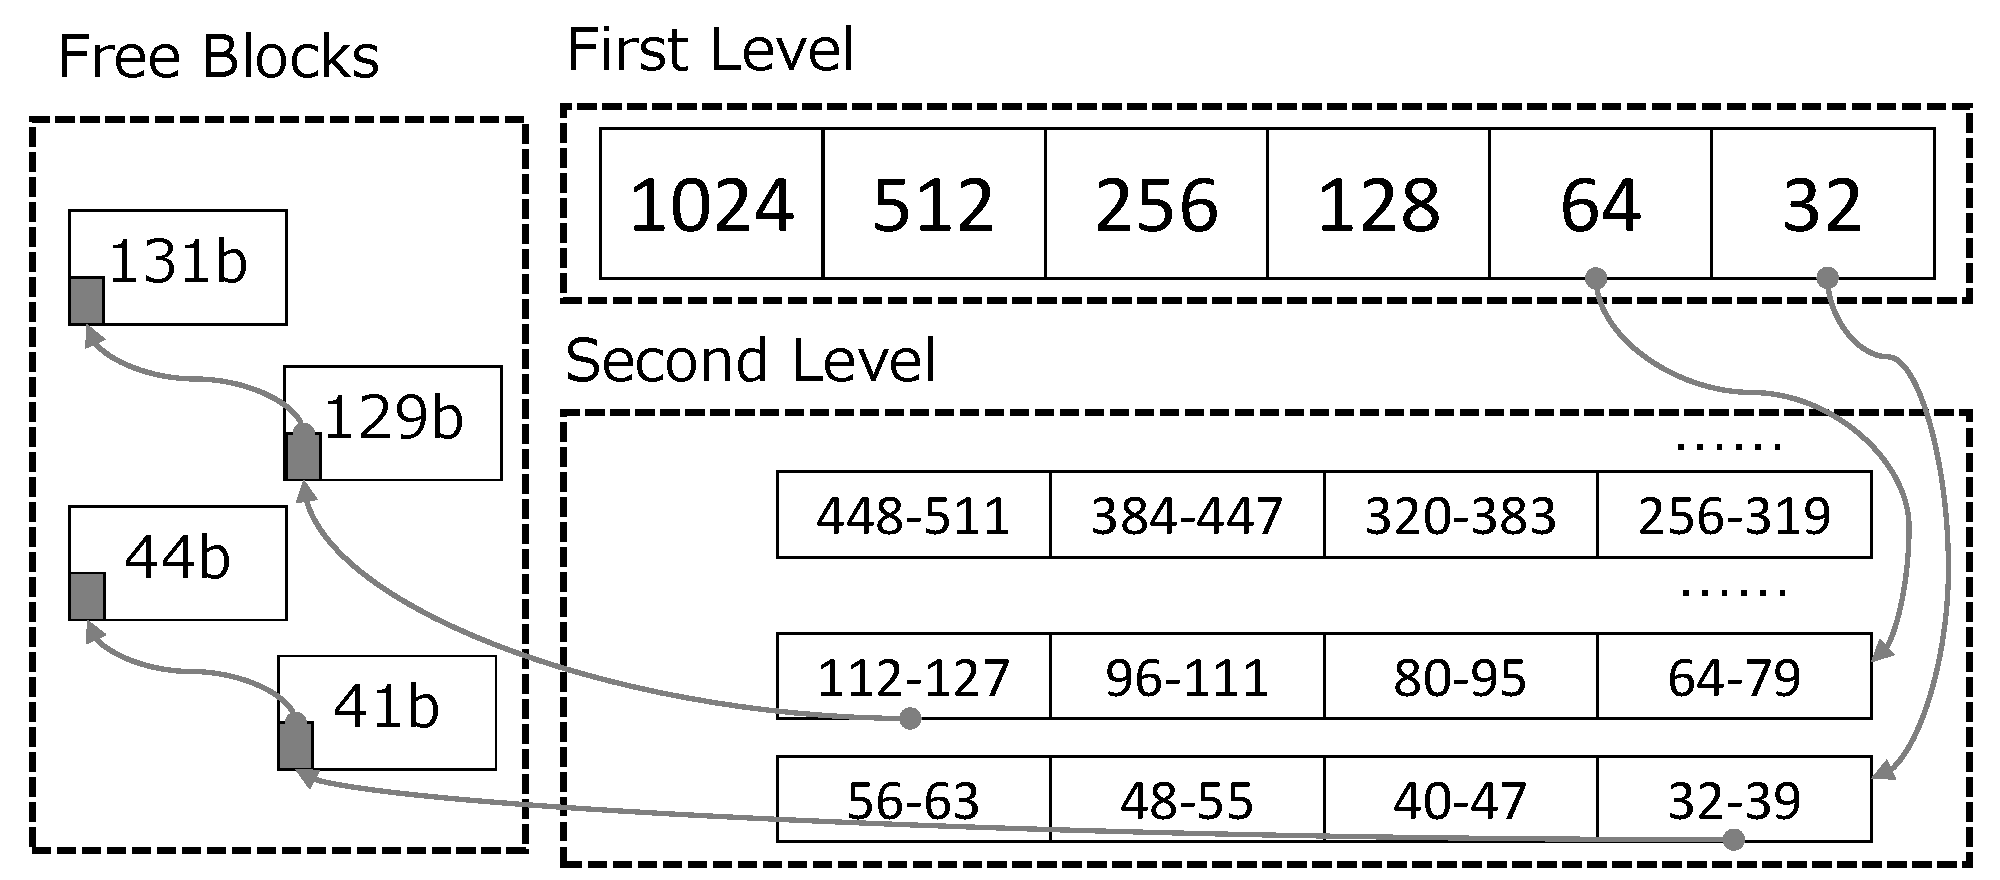
\includegraphics[width=8cm,clip]{figure/TLSF.pdf}
    \caption{TLSF Algorithm}
    \label{fig:TLSF}
\end{figure}


\subsubsection{Component Design of TLSF}

This section describes the component design of TLSF memory allocator.
In this research, we are using TECS to componentize TLSF.
The version of TLSF used is 2.4.6\footnote{http://www.gii.upv.es/tlsf/main/repo}.

\begin{figure}[t]
\centering
\begin{lstlisting}
signature sMalloc {
    int    initializeMemoryPool(void);
    void   *calloc( [in]size_t nelem,
                    [in]size_t elem_size );
    void   *malloc( [in]size_t size );
    void   *realloc( [in]const void *ptr,
                     [in]size_t new_size );
    void   free( [in]const void *ptr );
};
\end{lstlisting}
\caption{Signature description of memory management}  
\label{src:TLSFSignature}
\end{figure}

Fig.\ref{src:TLSFSignature} is a signature description for memory management used by the allocator.
It defines the memory pool initialization function {\it initializeMemoryPool}, memory allocation function {\it calloc}, {\it malloc}, {\it realloc}, and memory release function {\it free} as a signatures.

\begin{figure}[t]
\centering
\begin{lstlisting}
celltype tTLSFMalloc {
    [inline]
        entry  sMalloc  eMalloc;
    attr {
        /* memory pool size in bytes */
        size_t  memoryPoolSize;
    };
    var {
        [size_is( memoryPoolSize / 8 )]
            uint64_t   *pool;
    };
};
\end{lstlisting}
\caption{Celltype description of TLSF memory allocator component}  
\label{src:TLSFCelltype}
\end{figure}

The celltype description of the TLSF memory allocator component is shown in Fig.\ref{src:TLSFCelltype}.
An entry port, {\it eMalloc}, is connected to all components that perform memory management such as $malloc$ and $free$.
Here, {\it [inline]} is a specifier for Implementation as inline functions.
A memory pool size is defined as an attribute, and a pointer to a memory pool is defined as an variable.
Each component holds its own heap area, so even when calling functions for memory management at the same time in different threads, it is possible to operate without memory contention.

\begin{figure}[t]
    \centering
    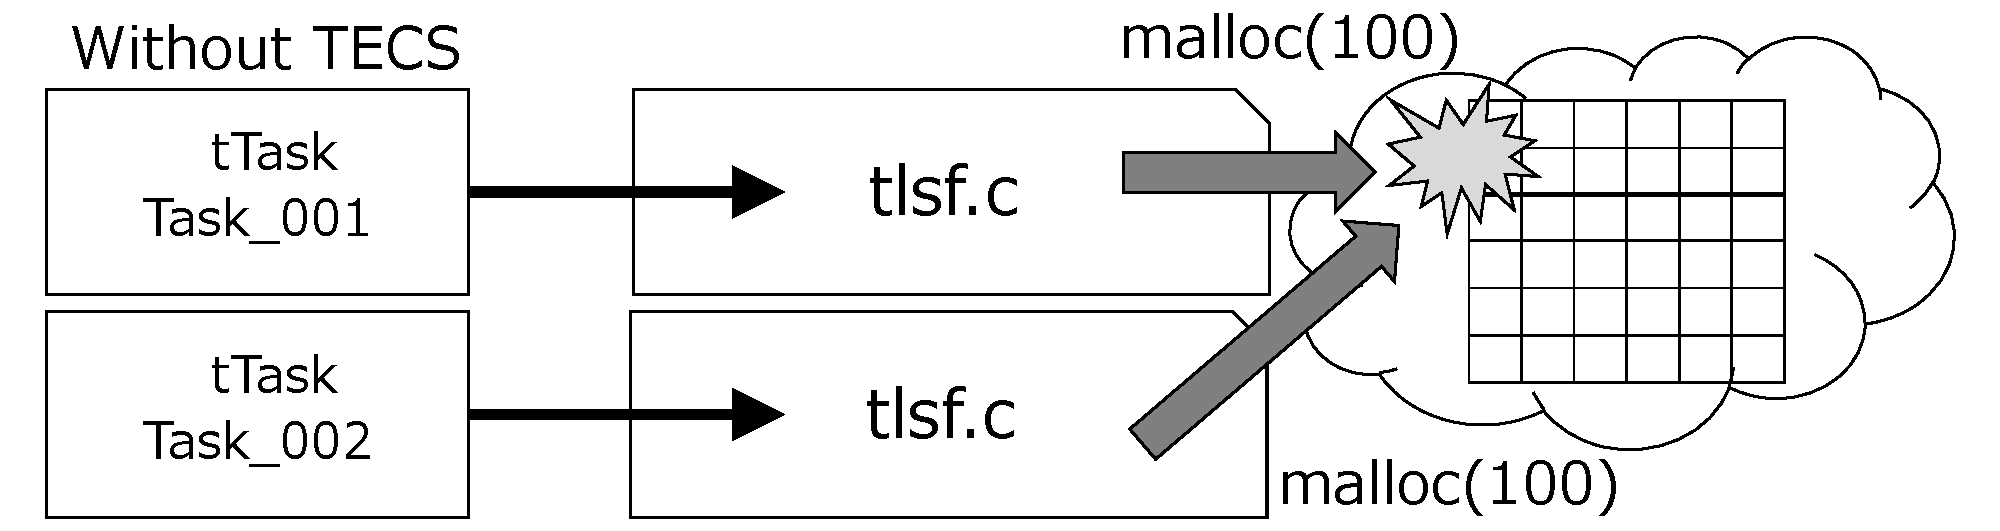
\includegraphics[width=8cm,clip]{figure/WithoutTECS.pdf}
    \caption{TLSF before componentization}
    \label{fig:WithoutTECS}
\end{figure}

\begin{figure}[t]
    \centering
    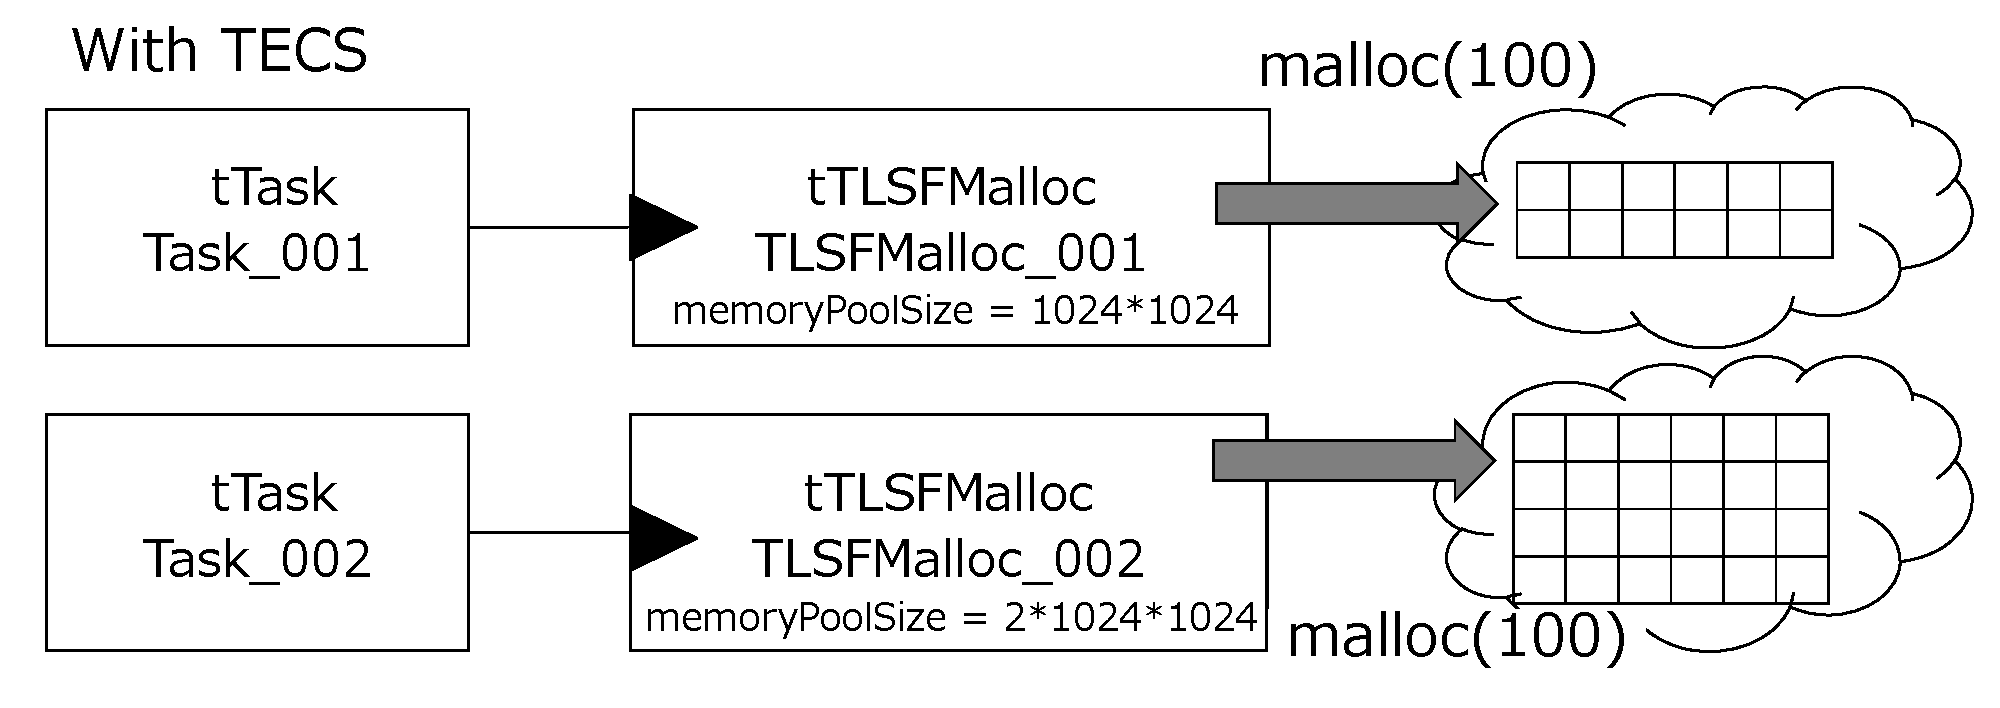
\includegraphics[width=8cm,clip]{figure/WithTECS.pdf}
    \caption{TLSF after componentization}
    \label{fig:WithTECS}
\end{figure}

As shown in Fig.\ref{fig:WithoutTECS}, since TLSF before componentization shares the heap area with multiple threads, if memory is allocated or released simultaneously from multiple threads, memory competition may occur in some cases.
In the research, TLSF is componentized using TECS as shown in Fig.\ref{fig:WithTECS}.
It is possible to operate in thread safe without exclusive control, because each component independently holds a heap area and manages memory within it. 

\begin{figure}[t]
\centering
\begin{lstlisting}
cell tTask Task_001 {
    cMalloc = TLSFMalloc_001.eMalloc;
};
cell tTLSFMalloc TLSFMalloc_001 {
    memoryPoolSize = 1024*1024; /* 1MB */
};
cell tTask Task_002 {
    cMalloc = TLSFMalloc_002.eMalloc;
};
cell tTLSFMalloc TLSFMalloc_002 {
    memoryPoolSize = 2*1024*1024; /* 2MB */
};
\end{lstlisting}
\caption{Build description of TLSF memory allocator component}
\label{src:TLSFBuild}
\end{figure}


\begin{figure}[t]
\centering
\begin{lstlisting}
void*
mrb_TECS_allocf(mrb_state *mrb, void *p, 
                  size_t size, void *ud)
{
    CELLCB	*p_cellcb = (CELLCB *)ud;
    if (size == 0) {
        //tlsf_free(p);
        cMalloc_free(p);
        return NULL;
    }
    else if (p) {
        //return tlsf_realloc(p, size);
        return cMalloc_realloc(p, size);
    }
    else {
        //return tlsf_malloc(size);
        return cMalloc_malloc(size);
    }
}
\end{lstlisting}
\caption{Example of TLSF memory allocator component}  
\label{src:TLSFC}
\end{figure}

Fig.\ref{src:TLSFBuild} shows the build description of the TLSF memory allocator component shown in Fig.\ref{fig:WithTECS}\footnote{Other call/entry ports, attributes, and valuables are actually described, but it is omitted here for the simplicity.}.
Two sets of task components and TLSF components are combined.
Each memory pool size can be configured as an variable (Lines 5 and 11 in Fig.\ref{src:TLSFBuild}).
Fig.\ref{src:TLSFC} is the part of the code actually calling the function of the TLSF memory allocator component.
The use part shows a function that the mruby VM allocates memory in the mruby on TECS framework\cite{par:mrubyonTECS}\cite{par:mrubyonTECS2} which is introduced in Section \ref{sec:mrubyonTECS}.
Lines 8 calls the {\it free} function of the TLSF memory allocator component.
{\it cMalloc\_} represents the name of the calle port (Lines 2 in Fig.\ref{src:TLSFBuild}).
Likewise, Lines 13 and 17 call the function for memory allocation.
The heap area of {\it TLSFMalloc\_001} component is used if the code of \ref{src:TLSFC} is executed in {\it Task\_001}, and if that is executed in {\it Task\_002}, the heap area of {\it TLSFMalloc\_002} component is used, respectively.
In this way, in the component-based development using TECS, it is possible to operate with the same code without modifying the C code, although the cells are different.


%4
\section{Evaluation}
\label{sec:Evaluation}


%5
\section{Related Work}
\label{sec:Related Work}


%6
\section{Conclusion}
\label{sec:Conclusion}


\begin{acknowledgment}

\end{acknowledgment}


%Reference
\bibliographystyle{ipsj_v2/UTF8/ipsjunsrt-e}
\bibliography{ref}

% \begin{biography}
% \profile{Taro Joho}{was born in 1970. He received his M.S. degree from
% Johoshori University in 1994.
% He joined
% the Information
% Processing Society of Japan in 1994.
% He is currently an associate professor at
% \mbox{Johoshori} University.
% His research interest is online
% publishing systems. He is a member of the IEEE and ACM\@.}
% %
% \profile{Hanako Shori}{was born in 1960. She received her M.E.\ and
% Ph.D.\ from Johoshori University in 1984 and 1987, respectively. She
% became an associate professor at Gakkai University in 1992 and a
% professor at Johoshori University in 1997. Her current research
% interest is online publishing systems. She received the Kiyasu Kinen
% award in 2010. She is a Board Member of the IPSJ and a member of the
% IEICE, IEEE-CS, and ACM\@.} 
% %
% \profile{Jiro Gakkai}{was born in 1970. He received his M.S.\ degree
% from Johoshori University in 1994 and has been engaged in the
% Information Processing Society of Japan since 1994. His research
% interest is online publishing systems. He is a member of the IEEE and
% ACM\@.}
% %
% \end{biography}

\end{document}
